\section{El \textit{Chana Monitoring System}}
\label{sect:intro}

El \CMS consta de dos módulos que se comunican a través de una conexión wifi estándar: el \MIE y el \MEE.

\begingroup

\setlength{\columnsep}{6pt}
\setlength{\intextsep}{6pt}

\begin{wrapfigure}{o}{0.5\columnwidth}
  \centering
  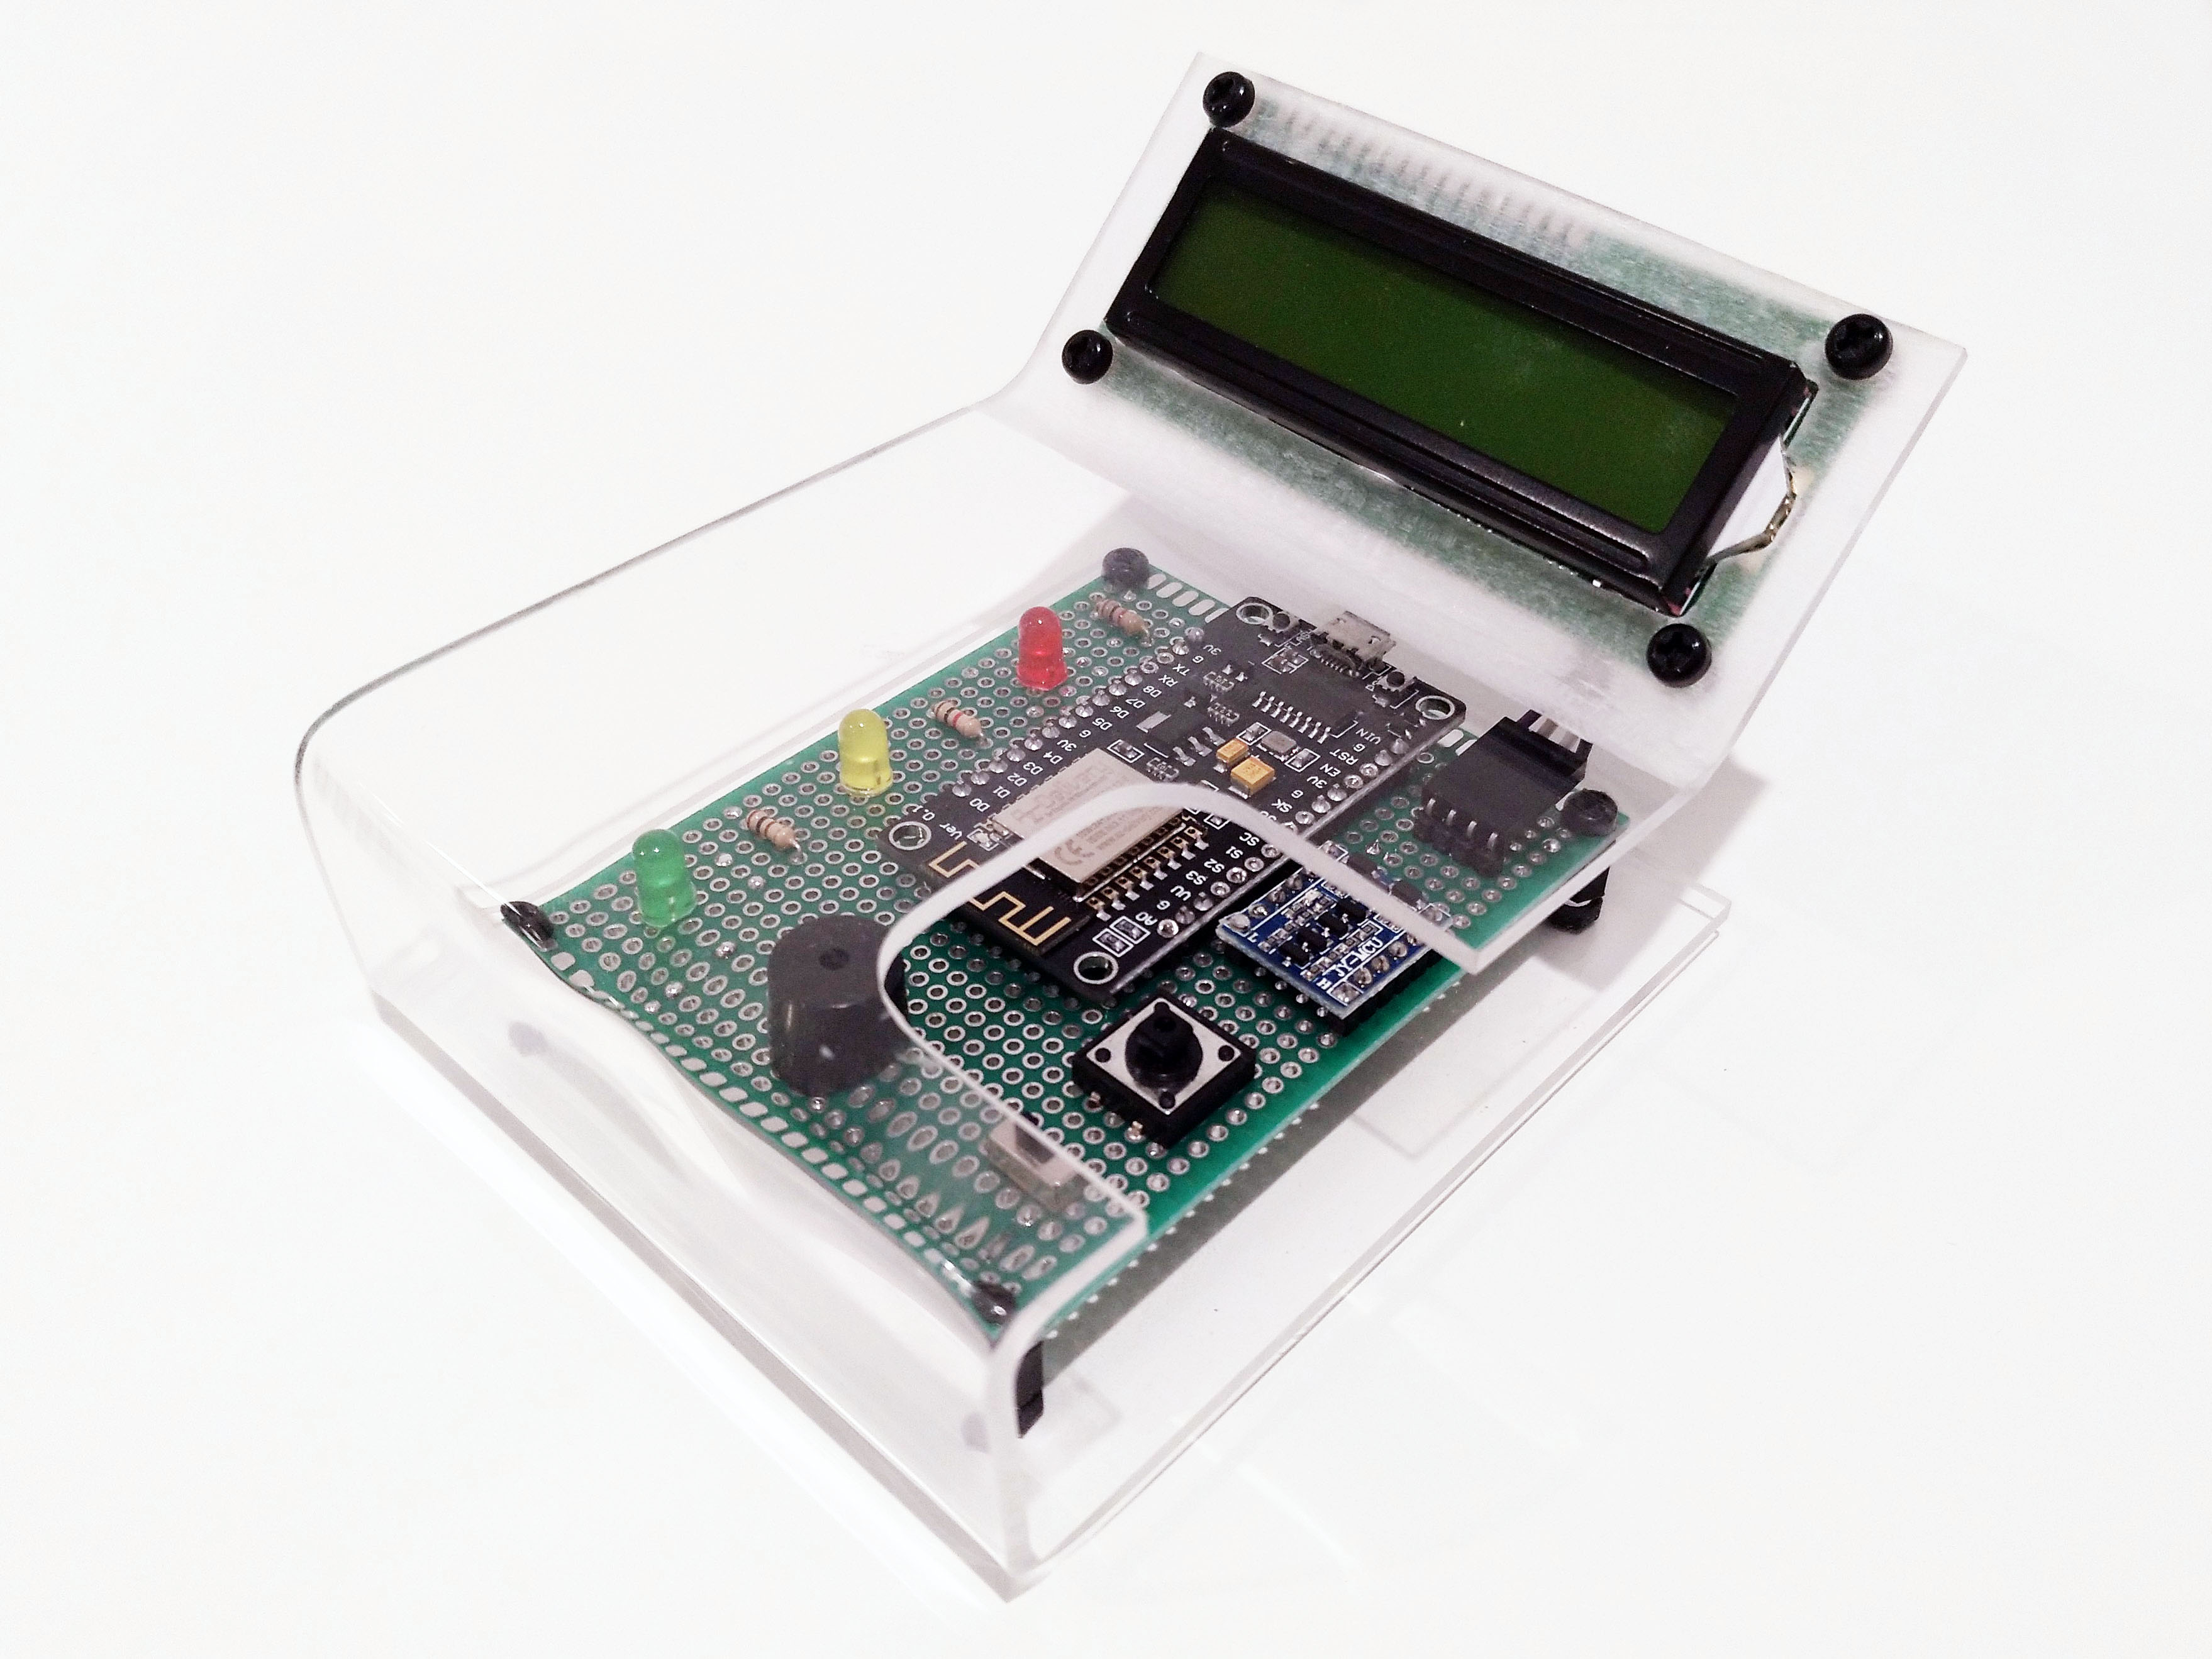
\includegraphics[width=0.5\columnwidth]{../photos/interior.jpg}
%   \caption{Módulo interior}
%   \label{fig:interior}
\end{wrapfigure}

El \MIE se debe colocar en el interior del hogar, preferiblemente en la habitación donde se encuentra la unidad interior de aire acondicionado que se desea monitorizar.
El \MI proporciona la información transmitida por el \ME, que monitoriza el estado del depósito de la unidad de aire acondicionado exterior, así como del ambiente (temperatura y humedad).
En caso de que el depósito se llene o se produca algún fallo, será el \MI el que lanzará los distintos avisos o alarmas a través de la pantalla, los testigos de colores, y la alarma sonora.
El \MI se alimenta mediante un adaptador de corriente USB estándar.

\begin{wrapfigure}{o}{0.5\columnwidth}
  \centering
  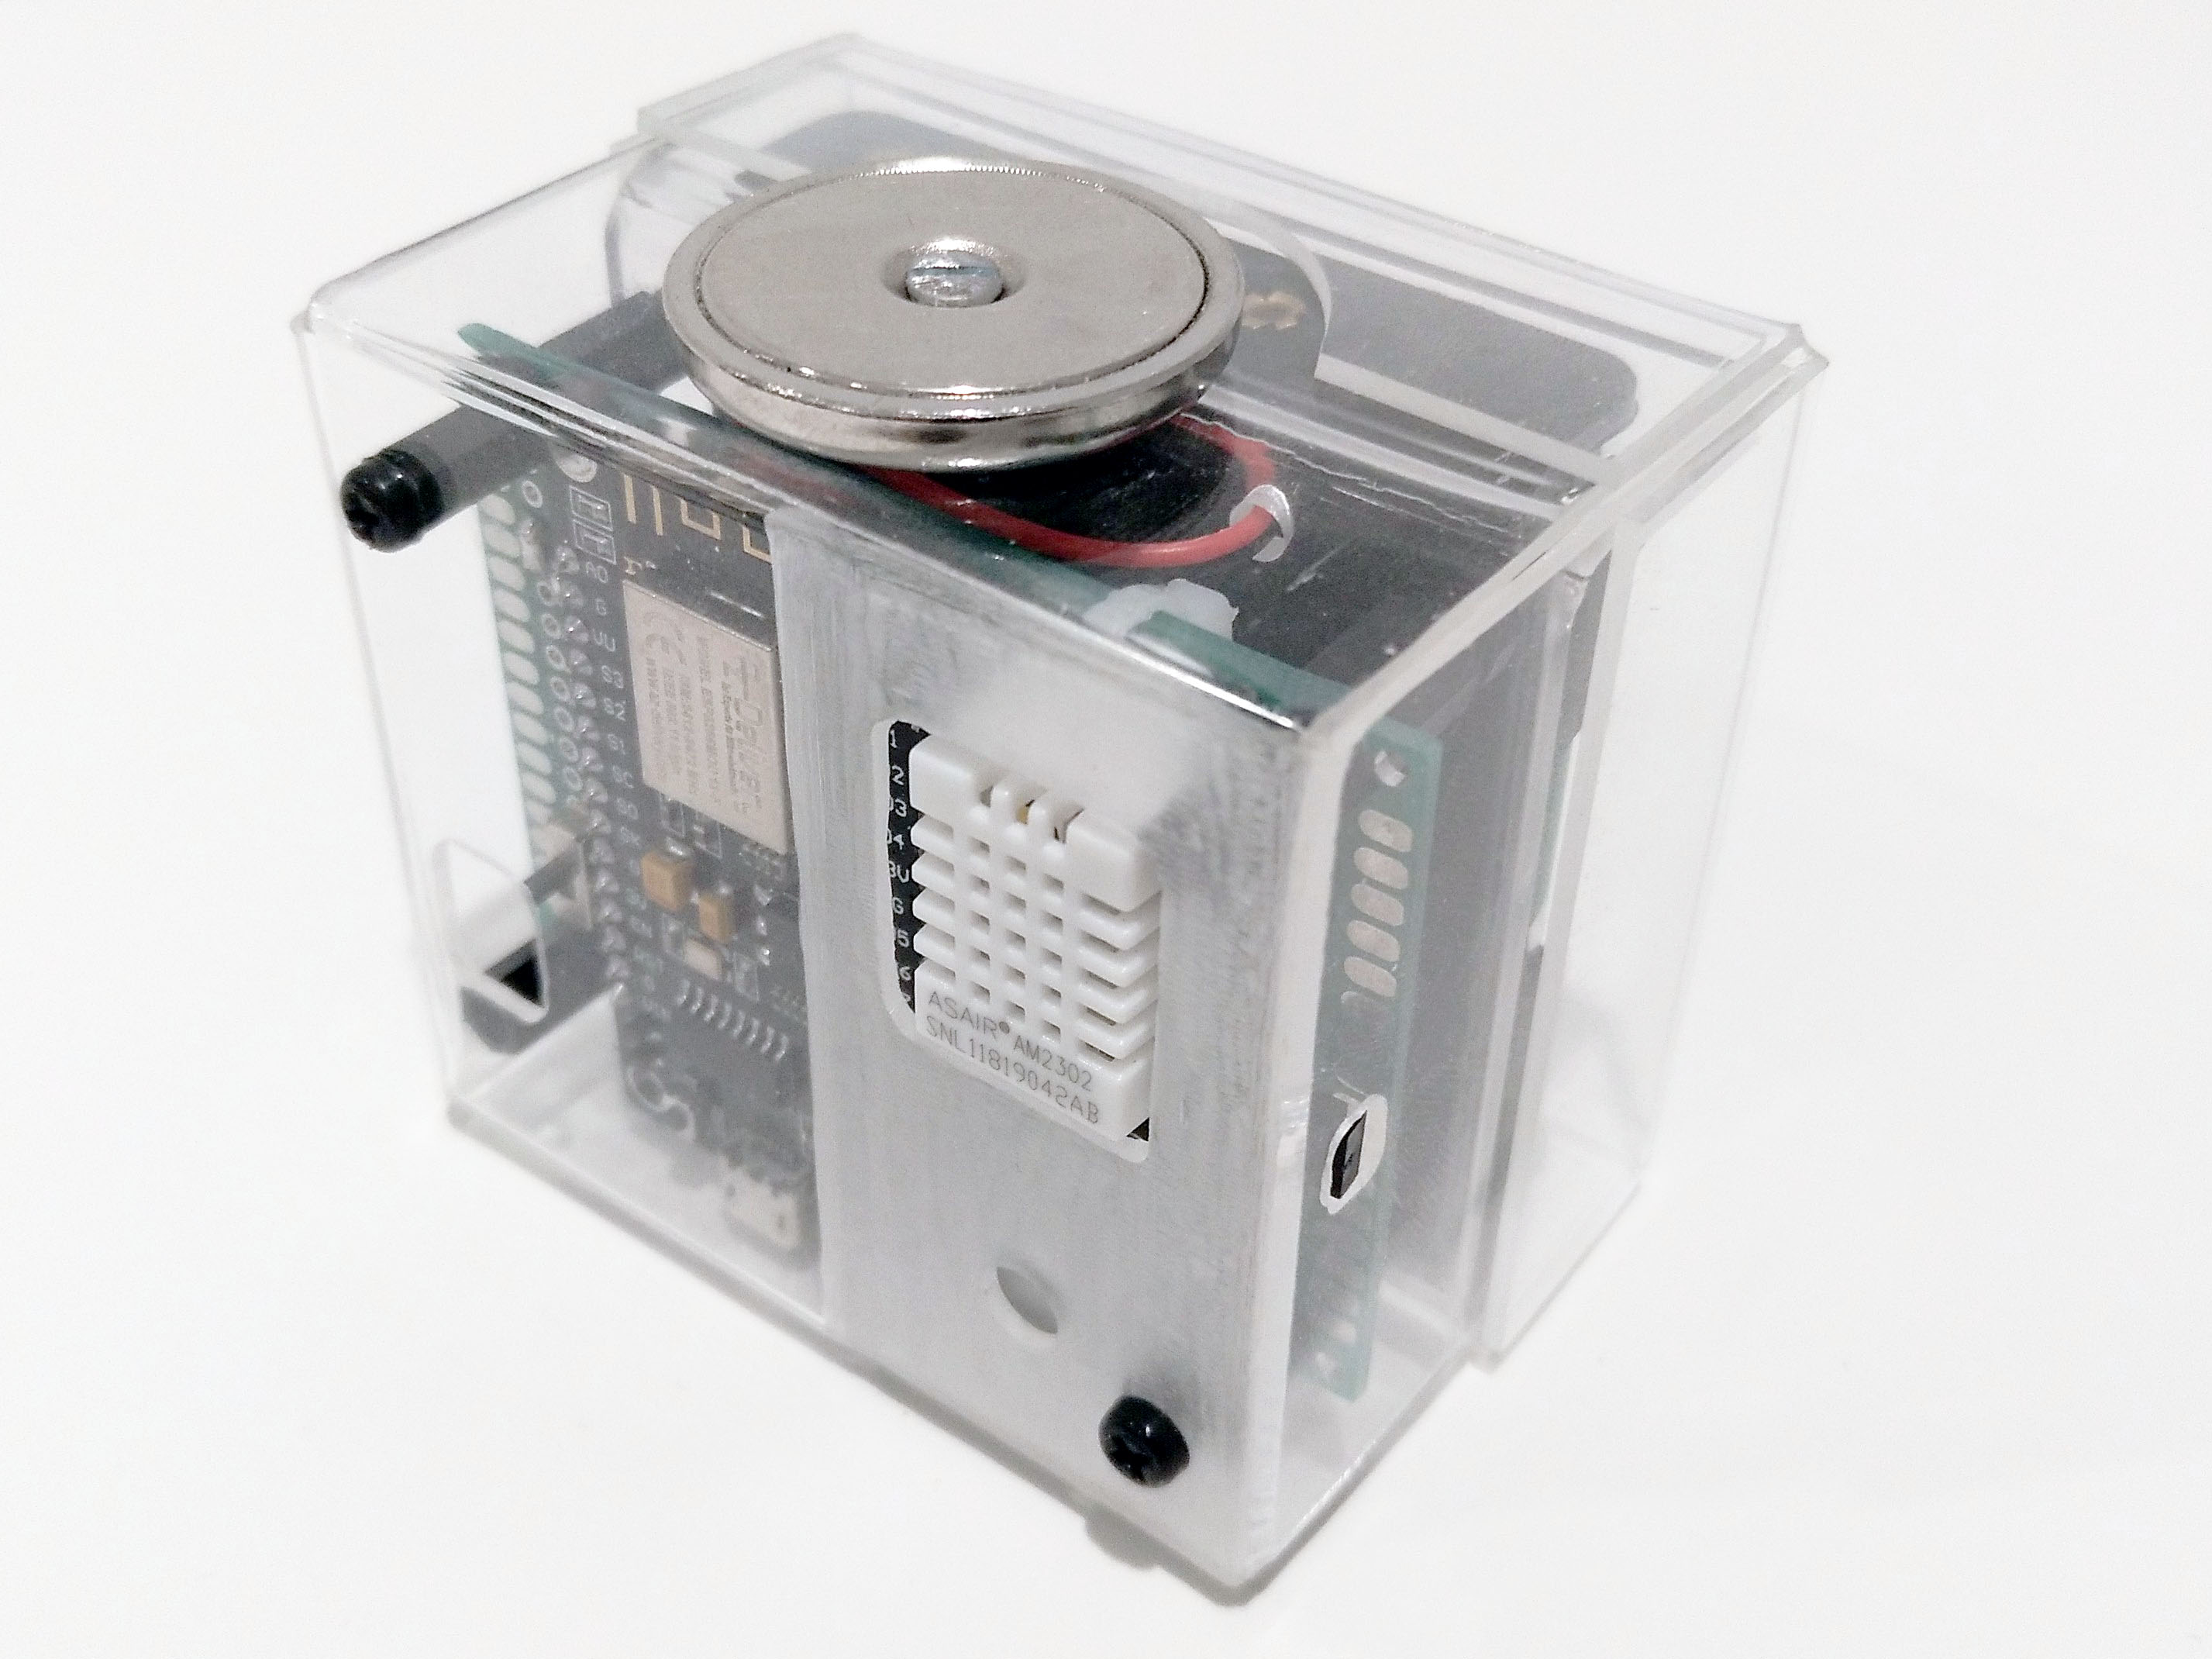
\includegraphics[width=0.5\columnwidth]{../photos/exterior.jpg}
%   \caption{Módulo exterior}
%   \label{fig:exterior}
\end{wrapfigure}

El \MEE recoge información mediante diferentes sensores, como el interruptor de flotador que debe introducirse dentro del depósito de agua a monitorizar.
Debe colocarse cerca de la unidad exterior de aire acondicionado en un lugar ventilado, alejado de la luz solar directa y del agua de lluvia.
El \ME dispone de un imán que permite fijarlo a la carcasa de la unidad exterior de aire acondicionado fácilmente.
El \MEE se alimenta mediante 4 pilas AA recargables de NiMH.

\importantbegin{No emplear pilas alcalinas}
El \MEE no se puede alimentar con pilas alcalinas estándares ya que proporcionan una tensión de salida de 1,5v. En todo caso se han de emplear 4 pilas AA recargables de NiMH (que dan una tensión de salida de 1,2v durante la mayor parte de su vida útil). El empleo de pilas alcalinas puede provocar daños permanentes por sobretensión en el \ME. 
\importantend

\endgroup

\subsection{Controles}
\label{sect:controles}

La figura~\ref{fig:interior-controls} muestra los principales controles del \MI:


\begin{enumeratecompact}
  \item[\textbf{\color{main}I1}:] Pantalla LCD.
  \item[\textbf{\color{main}I2}:] Luz de notificación de fallo.
  \item[\textbf{\color{main}I3}:] Luz de notificación de configuración.
  \item[\textbf{\color{main}I4}:] Luz de notificación de conexión.
  \item[\textbf{\color{main}I5}:] Botón de reinicio.
  \item[\textbf{\color{main}I6}:] Conexión de alimentación USB.
  \item[\textbf{\color{main}I7}:] Luz de notificación de actividad.
  \item[\textbf{\color{main}I8}:] Botón multiuso.
  \item[\textbf{\color{main}I9}:] Interruptor de la alarma sonora (\on = encendido, \off = apagado).
  \item[\textbf{\color{main}I10}:] Emisor de alarma sonora.
\end{enumeratecompact}

\begin{figure}
  \centering
  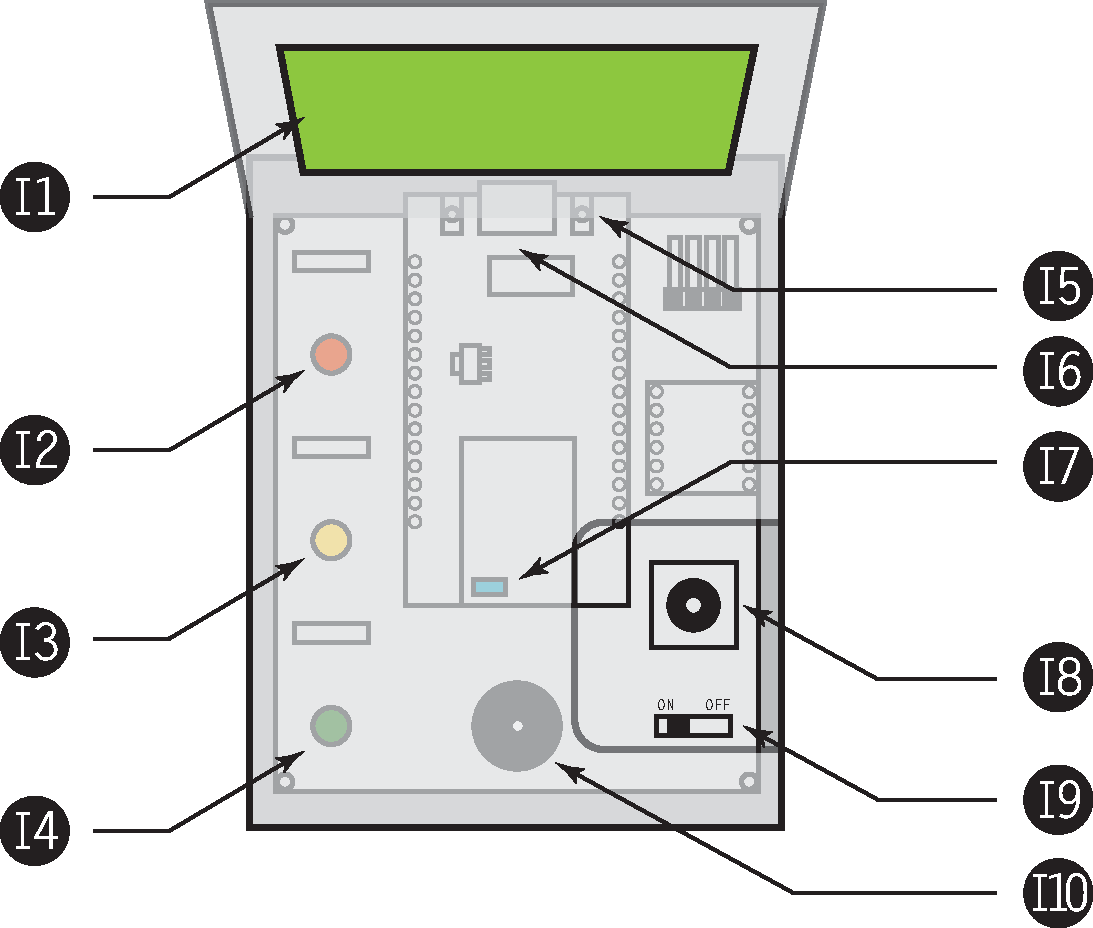
\includegraphics[width=0.8\columnwidth]{../design/interior-controls}
  \caption{Controles del módulo interior}
  \label{fig:interior-controls}
\end{figure}

La figura~\ref{fig:exterior-controls} muestra los principales controles del \ME:

\begin{enumeratecompact}
  \item[\textbf{\color{main}E1}:] Luz de notificación de actividad.
  \item[\textbf{\color{main}E2}:] Interruptor de encendido (\on = encendido, \off = apagado).
  \item[\textbf{\color{main}E3}:] Sensor de temperatura y humedad.
  \item[\textbf{\color{main}E4}:] Conexión para interruptor de flotador.
  \item[\textbf{\color{main}E5}:] Botón de configuración.
\end{enumeratecompact}

\begin{figure}
  \centering
  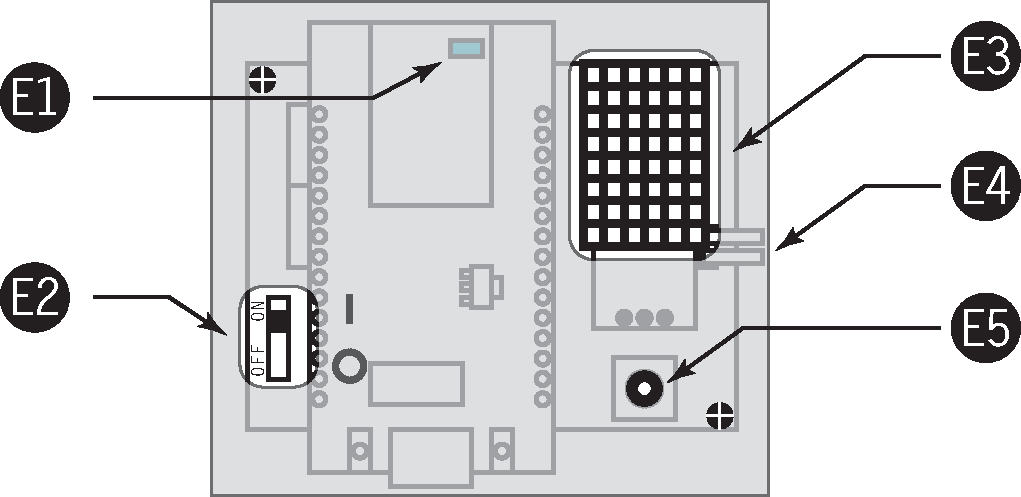
\includegraphics[width=0.8\columnwidth]{../design/exterior-controls}
  \caption{Controles del módulo exterior}
  \label{fig:exterior-controls}
\end{figure}